%%%%%%%%%%%%%%%%%%%%%%%%%%%%%%%%%%%%%%%%%%%%%%%%%%%%%%%%%
%                          导言区                        %
%%%%%%%%%%%%%%%%%%%%%%%%%%%%%%%%%%%%%%%%%%%%%%%%%%%%%%%%%
\documentclass[13pt]{ctexart} % 文档类
\usepackage{geometry} % 设置页面
\usepackage{graphicx} % 插图片
\graphicspath{{C:/Users/zheng/Desktop/mcm-2021/mcmdocs/figs/}}
\renewcommand{\figurename}{Figure} % 设置标题 重命名为英文
\renewcommand{\tablename}{Table}
\renewcommand{\contentsname}{Contents}
\usepackage{changepage} % 设置摘要页缩减
\usepackage{fontspec} % 便于修改字体
\usepackage{fancyhdr} % 设置页眉页脚
\usepackage{lastpage}
\pagestyle{fancy} % 清空页眉页脚
\usepackage[shortlabels]{enumitem} % 设置列表缩进
\usepackage{titlesec} % 设置修改默认的section标题大小
\titleformat*{\section}{\LARGE}
\titleformat*{\subsection}{\Large}
\titleformat*{\subsubsection}{\Large}
\usepackage{amsmath} % 使用数学宏包
\usepackage{amsfonts} % 使用数学字体
\usepackage{array} % 设置表格的列格式
\usepackage{booktabs} % 三线表宏包
\usepackage{etoolbox} % 设置参考文献不输出默认名
\usepackage{newtxtext}
\patchcmd{\thebibliography}{\section*{\refname}}{}{}{} % 引入网站作为参考文献
\usepackage[]{hyperref} % 设置引用且末尾不显示文档名
\usepackage{url} % 设置等宽的代码字体
%\setmonofont{IBM Plex Mono}
% 建议这个,但我系统没这个字体,且懒得折腾了 windows用户请
\setmonofont{Courier New}
% 颜色
\usepackage{xcolor} % 代码高亮方案宏包
\usepackage{listings}
\definecolor{CPPLight}  {HTML} {686868}
\definecolor{CPPSteel}  {HTML} {888888}
\definecolor{CPPDark}   {HTML} {262626}
\definecolor{CPPBlue}   {HTML} {4172A3}
\definecolor{CPPGreen}  {HTML} {487818}
\definecolor{CPPBrown}  {HTML} {A07040}
\definecolor{CPPRed}    {HTML} {AD4D3A}
\definecolor{CPPViolet} {HTML} {7040A0}
\definecolor{CPPGray}   {HTML} {B8B8B8}
\lstset{
	basicstyle=\ttfamily,
	breaklines=true,
	framextopmargin=50pt,
	frame=bottomline,
	columns=fixed,
    %numbers=left,                                       % 在左侧显示行号
	frame=none,                                          % 不显示背景边框
	backgroundcolor=\color[RGB]{255,255,255},            % 设定背景颜色
	keywordstyle=\color[RGB]{40,40,255},                 % 设定关键字颜色
	numberstyle=\footnotesize\color{darkgray},           % 设定行号格式
	commentstyle=\itshape\color[RGB]{0,96,96},                % 设置代码注释的格式
	stringstyle=\slshape\color[RGB]{128,0,0},   % 设置字符串格式
	showstringspaces=false,                              % 不显示字符串中的空格
	language=python,                                     % 设置语言
	morekeywords={alignas,continute,friend,register,true,alignof,decltype,goto,
		reinterpret_cast,try,asm,defult,if,return,typedef,auto,delete,inline,short,
		typeid,bool,do,int,signed,typename,break,double,long,sizeof,union,case,
		dynamic_cast,mutable,static,unsigned,catch,else,namespace,static_assert,using,
		char,enum,new,static_cast,virtual,char16_t,char32_t,explict,noexcept,struct,
		void,export,nullptr,switch,volatile,class,extern,operator,template,wchar_t,
		const,false,private,this,while,constexpr,float,protected,thread_local,
		const_cast,for,public,throw,std},
	emph={map,set,multimap,multiset,unordered_map,unordered_set,numpy,graph,path,append,extend,
		unordered_multiset,unordered_multimap,vector,string,list,deque,
		array,stack,forwared_list,iostream,memory,shared_ptr,unique_ptr,
		random,bitset,ostream,istream,cout,cin,endl,move,default_random_engine,
		uniform_int_distribution,iterator,algorithm,functional,bing,numeric,},
	emphstyle=\color{CPPViolet},
}

%%%%%%%%%%%%%%%%%%%%%%%%%%%%%%%%%%%%%%%%%%%%%%%%%%%%%%%%%
%                         正文区                         %
%%%%%%%%%%%%%%%%%%%%%%%%%%%%%%%%%%%%%%%%%%%%%%%%%%%%%%%%%
\begin{document}
%%%%%%%%%%%%%%%%%%%%%%%%%%扉页%%%%%%%%%%%%%%%%%%%%%%%%%%
\newgeometry{left=1in,right=0.75in,top=1in,bottom=1in}
% 第一页的字体为times new roman
\setmainfont{Times New Roman}
\thispagestyle{empty}
% 扉页抬头

\vspace*{-16ex}
\centerline{\begin{tabular}{*3{c}}
        \parbox[t]{0.3\linewidth}{
            \begin{center}\textbf{Problem Chosen}\\ \Large \textcolor{red}{B}\end{center}
        }
         & \parbox[t]{0.3\linewidth}{\begin{center}\textbf{2021\\ MCM/ICM\\ Summary Sheet}\end{center}}
         & \parbox[t]{0.3\linewidth}{\begin{center}\textbf{Team Control Number}\\ \Large \textcolor{red}{2120710}\end{center}} \\
        \hline
    \end{tabular}}

\vspace*{3ex}

% 大标题
{\centering\fontsize{18}{16}\selectfont\textbf{{Fighting Wildfire with Unmanned Aerial Vehicle}}

    % summary
    \vspace{10pt}
    \fontsize{13}{10}\selectfont\textbf{{Summary}}\par}
\vspace{10pt}

% summray正文
\fontsize{13}{12.5}\selectfont %summary正文字体 13 pt
\begin{adjustwidth}{1cm}{1cm}
    \indent { }{ }{ }{ }{ }{ }
    在这里写summary

    % 关键词
    \vspace{15pt}
    \textbf{key words} : 关键词1; 关键词2; 关键词3
\end{adjustwidth}

%%%%%%%%%%%%%%%%%%%%%%%%%%MEMO页%%%%%%%%%%%%%%%%%%%%%%%%%%
\newpage
% 开始写 memo 信
% 更换字体为 palatino 也可以不换
\setmainfont[
    BoldFont       = texgyrepagella-bold.otf ,
    ItalicFont     = texgyrepagella-italic.otf ,
    BoldItalicFont = texgyrepagella-bolditalic.otf ]{texgyrepagella-regular.otf}
\newgeometry{left = 3.5cm, right = 3.5cm}
\thispagestyle{empty}
% memo标题+信息
{\centering \fontsize{18pt}{14pt}\selectfont \textbf{Budget Request}\par}

\noindent FROM: Team {} 2120710 , MCM\\
\noindent To: The group of Governors\\
\noindent Date: February 8, 2020
% request正文
\vspace{10pt}
\\
这里是br正文。

% 信多出一页,清理页眉页脚
\thispagestyle{empty}
% 信的结尾
{\raggedleft
    Sincerely yours,\\
    MCM Team 2120710\par
}

%%%%%%%%%%%%%%%%%%%%%%%%%%目录页%%%%%%%%%%%%%%%%%%%%%%%%%%
\newpage
\thispagestyle{empty}
\tableofcontents
%%%%%%%%%%%%%%%%%%%%%%%%%%正文页%%%%%%%%%%%%%%%%%%%%%%%%%%
\newpage
% 目录页后面是第一页
\setcounter{page}{1}

% 开始写正文
% 设置正文的页边距
\newgeometry{top=3cm, left=3.5cm, right=3.5cm}
% 设置正文的页眉页脚
\fancyhf{}
\fancyhead[C]{ }
% 此处修改右上角页码
\fancyhead[R]{Page \thepage\ of \pageref{LastPage}}
\fancyhead[L]{Team \# 2120710}
\fancyfoot[C]{\bfseries\thepage}
%%%%%%%%%%%%%%%%%%%%%%%%%%%%%%%%%%%%%%%
%% Introduction
\textbf{\section{Introduction}}
% .1
\textbf{\subsection{Restatement of the Problem}}
Many people...Therefore we are facing the following problems:
\begin{itemize}
    \item aaaaaa
    \item aaaaaaa
\end{itemize}

% .2
\textbf{\subsection{Our Works}}
\begin{itemize}
    \item aaaaaaa
    \item aaaaaa
\end{itemize}
\fancyfoot[C]{\bfseries\thepage}
%%%%%%%%%%%%%%%%%%%%%%%%%%%%%%%%%%%%%%%
%% Assumptions and Notations
\textbf{\section{Assumptions and Notations}}
\vspace{-10pt}
% Assumptions
\textbf{\subsection{Assumptions}}
Due to the lack of necessary data, we make the following assumptions to help us perform modeling:

\begin{itemize}[itemsep=0.3ex, leftmargin=1.2cm]
    \item[1.] The circumstance remain unchanged in the time interval we investigated.
    \item[2.] We omit the possibility of any other kinds of aerial vehcle or flying creature hitting our UAV.
    \item[3.] Accroding to Bureau of Meteorology of Australian Government, litghting is the major causation of bushfire in some area, Victoria included. \cite{ref02} Based on this fact, we evaluat the possibility for a certain place to catch fire with the possibility of a lightning to occour there.
    \item[4.]  We adopt the Equal Possibility Hypothesis when our UAVs are patrolling for the purpose of monitoring any outbreak of fire.Under this hypothesis, an area of high possibility to catch fire indicates the frequency of fire outbreak here is high, thus the command center should pay closer attention to this area to alarm fire outbreaks timely.
    \item[5.] All UAVs are equipped with a timer.
    \item[6.] All UAVs are directed by a preprogrammed system given by us, which means they are all automatic.
    \item[7.] Staffes are always available in any charging stations, which guarantees the UAVs will always work in the stanterd situation.
    \item[8.] A drone can carry either a set of thermal imaging cameras and telemetry sensors or a radio repeater. The former combination can and can only detect any fire outbreak, while the latter can and can only extend the valid zone of radio wave signals.
\end{itemize}
% Notations
\textbf{\subsection{Notations}}
% coordinate system
\textbf{\subsubsection{\textit{ijk}-coordinate system}}
Before illustrating the notations for model construction, we would like to introduce a special coordinate system called \textbf{\textit{ijk}-coordinate system}\cite{uber-h3-doc}, which was first proposed by Uber Technologies Inc.
Discrete hexagon planar grid systems naturally have 3 coordinate axes spaced $120^{\circ}$ apart. We refer to such a system as an \textit{ijk} coordinate system, for the three coordinate axes $i$, $j$, and $k$.

\begin {figure}[h]
\centering % 居中显示
%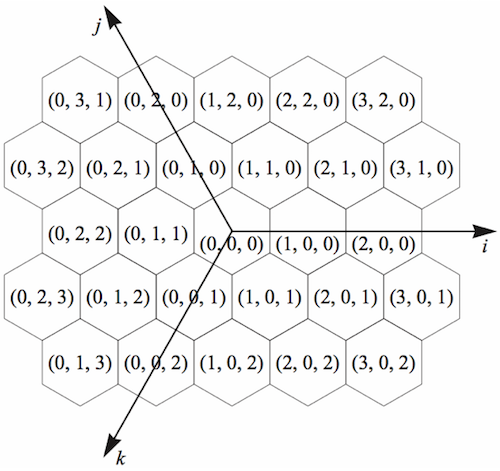
\includegraphics[width=15cm,height=12cm]{ijkp.png}
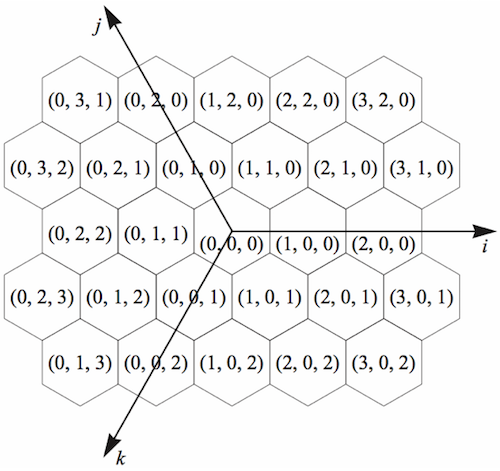
\includegraphics[scale=0.4]{ijkp.png}
\caption{One possible map example that using the \textit{ijk} coordinate system} % 标题
\end {figure}

% Notations
\textbf{\subsubsection{Notations}}
Here are all the notations and their meanings in this paper.
\begin{table}[h]
    \centering
    \caption{Notations used in model construction}
    \vspace{3pt}
    \begin{tabular}{>{\centering\arraybackslash}p{6em}>{\centering\arraybackslash}p{30em}}
        \toprule % 绘制第1条线
        Notation         & Meaning                                      \\
        \midrule % 绘制第2条线
        $M
        (i,t)$           & Location of the $i$-th drone
        \uppercase\expandafter{\romannumeral1} at time $t$              \\
        $R
        (j,t)$           & Location of the $j$-th drone
        \uppercase\expandafter{\romannumeral2} at time $t$              \\
        $h
        (x,y,z)$         & Elevation of the point $(x,y,z)$             \\
        $S
        (x,y,z)$         & Fire history of the point $(x,y,z)$
        in the passed $5$ years                                         \\
        $a_i
        (x,y,z)$         & Fire history of the point $(x,y,z)$
        in the $2020-i$-th year,
        $i\in [1,5] \cap \mathbb{N} $                                   \\
        $F(x,y,z) $      & Vegetative and structural
        condition of the point$(x,y,z)$                                 \\
        $S(i,x,y,z,t)$   & Strength of the signal from the $i$-th drone
        at point $(x,y,z)$ at time $t$                                  \\
        $E
        (x,y,z,N)$       & Supervisory density of the point $(x,y,z)$
        when there are $N$ drones in the field                          \\
        $Slope
        (x,y,z)$         & Maximum slope of the point $(x,y,z)$         \\
        $\gamma$         & Factor used to calculate the weight
        of slope in causing bushfire                                    \\
        $\beta
        (x,y,z)$         & Weight of slope in causing bushfire          \\
        $\omega
        (x,y,z)$         & Decreasing rate of signal at point $(x,y,z)$ \\
        $\alpha$         & Elevational factor                           \\
        $Chg
        (q,x,y,z)$       & Location of the $q$-th charging station      \\
        $V_{max}$        & Maximum flying velocity of a drone           \\
        $N_{\text{SSA}}$ & Amount of drone
        \uppercase\expandafter{\romannumeral1}                          \\
        $N/rep$          & Amount of drones
        \uppercase\expandafter{\romannumeral2}                          \\
        $PF$             & Power consumption for a flying drone         \\
        $PH$             & Power consumption for a hovering drone       \\
        $t_{fl}
        (t,l)$           & Flight time of the $l$-th drone
        until time $t$                                                  \\
        $t_{hov}
        (t,l)$           & Hovering time of the $l$-th drone
        until time $t$                                                  \\
        $T$              & Duration of a day (i.e. $1440 \min$)         \\
        $t$              & Current time                                 \\
        $Br$             & Total battery power of a drone               \\
        $Ini$            & Location of the EOC                          \\
        \bottomrule
    \end{tabular}
\end{table}
%%%%%%%%%%%%%%%%%%%%%%%%%%%%%%%%%%%%%%%
%% Model Construction
\textbf{\section{Model Construction}}
blablablabla
%%%%%%%%%%%%%%%%%%%%%%%%%%%%%%%%%%%%%%%
%% Conclusion
\textbf{\section{Conclusion}}
We build a.....interesting findings:

\begin{itemize}
    \item aaaaaaa
    \item aaaaaaa
\end{itemize}

%%%%%%%%%%%%%%%%%%%%%%%%%%参考文献%%%%%%%%%%%%%%%%%%%%%%%%%%
% 因为不输出此部分到目录 \addcontentsline{}{}{}是添加此标题到目录
\newpage
\textbf{\section*{References}\addcontentsline{toc}{section}{References}}
\fancyhf{}
\fancyhead[R]{ }
\fancyhead[L]{ }
\bibliography{books}
\Large
\bibliographystyle{IEEEtran}
%%%%%%%%%%%%%%%%%%%%%%%%%%附录%%%%%%%%%%%%%%%%%%%%%%%%%%
\newpage
\textbf{\section*{Appendices}\addcontentsline{toc}{section}{Appendices for Code and Data}}
\fontsize{13pt}{12.5pt}\selectfont
Here is Code we used in our model, which python is the main development language.
\vspace{7pt}
\textbf{\subsection*{Appendices A}}

fooooo

\end{document}